%===================================== CHAP 4 =================================

\chapter{Neural Linear Bayesian Regression Model}\label{ch:bdqn}

A major drawback of the methods discussed in chapter \ref{ch:linear} is that they are all linear models. These cannot perform well in environments with complex non-linear relationships between state-action pairs and Q-values without significant feature engineering. Recent developments in the RL field focus on deep RL\citep{mnih_2015, mnih_2016,silver_2017} where neural networks are used as encode these relationships have allowed successfull results on complex games. As such it it would be beneficial to be able to combine the methods from chapter \ref{ch:linear} with more complex models. This chapter attempts this and tests the new model on multiple complex environments with comparisons to other popular deep RL methods.

\section{Combining Bayesian Q-learning with Neural Networks}

\subsection{Neural Linear Model}

Without significant feature engineering a linear model cannot generalize to more complex non-linear relationships between state-action pairs and their Q-values. However using bayesian methods with non-linear models can be difficult and computationally heavy. \cite{carlos_2018} compared a large array of bayesian models on a set of bandit environments. They found that accurate complex models often performed worse than simpler approximate methods. The suggested reason for this is that complex models require more data and training to acheive reasonable variance estimates. Since RL is an online task this can lead to miscalibrated variance early on in the training process that leads to worse results.

Emperically \cite{carlos_2018} finds what they coin as a neural linear model to work best. The model consists of using a neural network as a basis function that is used as the covariates to a linear bayesian regression model. This is equivalent to rewriting the regression task to 

\begin{equation*}
	Q = \phi(X)\beta + \varepsilon \quad \text{where} \quad \varepsilon \sim N(0,\sigma^2)
\end{equation*}

where $\phi(X)$ is the neural networks output given an input $X$. The error in the bayesian regressions point estimates is backpropagated through the neural network to learn a useful basis function. Note that this means the bayesian regression no longer incorporates all the uncertainty since the above assumes no uncertainty in the $\phi(X)$ encoding. \cite{carlos_2018} suggests that error that comes with this assumption is counteracted by the models stable uncerainty estimates.

This setup allows the application of the methods discussed in chapter \ref{ch:linear} in more complex environments. It is also this method \cite{azziz_2018} follows in their application of the BN model to more complex models.

\subsection{Bayesian DQN Models}

Based on the results of \cite{carlos_2018} this thesis attempts to combine neural networks and the BNIG model through a neural linear setup. To start off a summary of the archicture used in \cite{azziz_2018}, called the BDQN, is provided. This is used as a base which will modified to fit with the BNIG model and thus allow for better variance propagation.

The BDQN architecture starts with the same archicture as the standard DQN architecture\citep{mnih_2015}. The final layer of a DQN is a linear layer which means it can be replaced by any linear model. \cite{azziz_2018} replaces this with a BN model and uses the MAP target for both without considering the possibility of sampling the target. The neural network is trained using the loss function

\begin{equation*}
	\theta = \theta - \alpha\nabla_\theta\big(Q_t - [\mu_n^T\phi_\theta(x_t)]\big)^2.
\end{equation*}

 The only difference to a regular neural network is that the networks output estimate is replaced by the MAP estimate of $\beta$. One could replace the MAP estimate by samples from the posterior $Q$. However as the network does not consider the variance of the target it is less computationally expensive and more stabalizing to use the MAP. The pseudocode for this update is

\begin{algorithm}[H] 
    \caption{BDQN Network Training} 
    \label{alg:BDQN_train} 
        \If{$t \; \textbf{mod} \; T_{train}$ == $0$}{ 
            Sample random minibatch of transitions $(s_j, a_j, r_j, s_{j+1})$ from $\mathcal{D}$ \\ 
            $a' = \argmax_a \big(\phi(s_t)\mu_a\big)$ for each transition \\ 
            Set $y_j = \begin{cases} 
                r_j \quad \text{for terminal} \quad s_{j+1}\\ 
                r_j + \gamma\phi^*(s_t, a')\mu^*_{a'} \quad \text{else} 
            \end{cases}$ \\ 
            Optimize the network weights over the Huber loss (equation \ref{eq:huber_loss}) 
        } 
\end{algorithm}

The BN model is trained using the posterior updates described in chapter \ref{ch:linear} in equation \ref{eq:known_noise_posterior_update}. Since the BN model does keep track of variance one could consider using a sample targert rather than the MAP target in this case. However it has already been shown that in the linear case using a sampled target over a MAP target has no effect on the final estimate as it does not propagate uncerainty.

These two training processes do not have to happen sequentially. In \cite{azziz_2018} the neural network is updated as frequently as in the original DQN implementation, while the bayesian regression trained from scratch every 10,000 steps on either 100,000 datapoints or the entire replay buffer if it contains less. This is done to handle the non-stationarity of the task. 

\subsection{From BDQN to BNIG DQN}

The downside retraining the bayesian regression is that this is computational heavy, especially considering that the final layer in the neural network consists of 512 neurons, meaning the update requires matrix arithmetic with a 512 by 512 matrix. On top of this using a BNIG model requires the target Q-values to be sampled from the posterior. This means every 10,000 steps 100,000 new samples must be drawn which requires a new set of matrix arithmetic of the same magnitude. Instead this thesis considers the exponential forgetting method. However implementing this requires some extra considerations to ensure that the model remains stable.

Recall that the classic DQN has one online network that is updated each training step and one target network that is updated occaisonally to match the online network. \cite{mnih_2013} found that using this target network to calculate the regression target helped stabalize the algorithm.

With exponential forgetting the bayesian regression is trained continuosly. However, using the online bayesian regression method to calculate targets based on the output from the target network will lead to instability. The regression model can train on thosands of datapoints from the online network between network syncs. Using different network encodings for the target and prediction with the same bayesian regression will lead to a different results which will artificially increase the loss. An increased loss leads to larger network changes which amplifies the effect leading to instability.

To deal with this issue the same setup that is used for the networks is used for the regression models. Two bayesian regression models are created, one online and one target. The target model is used to calculate the target action-values while the online model is used for decision making. The target model is then updated to the parameters of the online model when the target network is updated. This decreases the loss and resulted in a stable network. The pseudocode for this update is seen in algorithm \ref{alg:bnig_train}. Note that the $^*$ notation denotes values from the target parameters and $\varepsilon_a$ is a sample from $N(0,\sigma^2_a)$.

\begin{algorithm}[H]
    \caption{BNIG training}
    \label{alg:bnig_train}
        \If{$t \; \textbf{mod} \; \textit{batch size} == 0$}{
            Sample random minibatch of transitions $(s_j, a_j, r_j, s_{j+1})$ from $\mathcal{D}$ \\
            Sample $\beta_a, \sigma_a$ for $a\in \mathcal{A}$ for each transition\\
            $a' = \argmax_a \bigg(\phi(s_t)\beta_a + \varepsilon_a\bigg)$ for each transition \\
            Sample $\beta^*_{a'}, \sigma^*_{a'}$ for $a'$ in each transition \\
            Set $y_j = \begin{cases}
                r_j \quad \text{for terminal} \quad s_{j+1}\\
                r_j + \gamma\bigg(\phi^*(s_t, a')\beta^*_{a'} + \varepsilon^*_{a'}\bigg)\quad \text{else}
            \end{cases}$ \\
            Update BNIG model parameters using posterior update equation \ref{eq:unknown_noise_posterior_update}
        }
\end{algorithm}

With this approach the only required change to transform the BDQN setup to a BNIG method is to swap out the BN model used in the BDQN with the BNIG model and sample action-values from the posterior for both the online and target models. The resulting algorithm is summarized in the pseudocode below.

\begin{algorithm}[H]
    \caption{BNIG DQN}
    Initialize variables according to algorithm \ref{alg:bnig_init}\\
    \For{episode = 1, M}{
        Initialize environment\\
        $s_1 = $ initial environment state\\
        
        Sample $\beta_a, \sigma_a$ for $a\in \mathcal{A}$\\
        \For{t=1, T}{
            $a_t = \argmax_a \bigg(\phi(s_t)\beta_a + \varepsilon_a$\bigg) \\
            Execute action $a_t$ and observe reward $r_t$ and state $s_{t+1}$ \\
            Store transition $(s_t, a_t, r_t, s_{t+1})$ in $\mathcal{D}$\\
            Train online network using algorithm \ref{alg:bdqn_train}\\
            Train online model using algorithm \ref{alg:bnig_train} \\
            \If{$t \; \textbf{mod} \; T_{sync}$ == $0$}{
                Set target network weights to online network weights\\
                Set target BNIG parameters to online BNIG parameters.
            }
        }
    }
\end{algorithm}

Here $T_{sync}$ is a hyperparameter that defines how often to sync the online and target network and model. Once again $\varepsilon_a$ represents a sample from $N(0,\sigma^2_a)$. The initialization process in algorithm \ref{alg:bnig_init} sets up the models, networks and experience buffer required.

\begin{algorithm}[H]
    \caption{BNIG DQN Initialization}
    \label{alg:bnig_init}
    Initialize experience buffer $\mathcal{D}$ with capacity $N$\\
    Initialize neural network $\phi$ with random weights $\theta$\\
    Initialize target neural network $\phi*$ with weights $\theta^*=\theta$\\
    Initialize $|\mathcal{A}|$ BNIG models with priors $\mu_a = zeros(p,1)$, $\Sigma_a = diag(p,p)$, $\alpha_a = 1$, $\beta_a = 0.01$
    Initialize target BNIG models with priors $\mu^*_a = \mu^*_a$, $\Sigma^*_a = \Sigma^*_a$, $\alpha^*_a = \alpha^*_a$, $\beta^*_a = \beta^*_a$.
\end{algorithm}

\section{BNIG DQN Results}

In this section the BNIG DQN is tested on a variety of environments and compared to a regular DQN.

To ensure a correct implementation of the DQN and a fair comparison to the BNIG DQN the python package Dopamine\citep{castro_18} was used. This package contains an implementation of a DQN that matches the baselines of the \cite{mnih_2015}. The BNIG DQN was implemented ontop of this DQN implementation.

The Dopamine package has hyperparmeters for the DQN on many of the tested environments. In some of the environments no hyperparemeters were provided or the ones given performed badly. In these cases, to avoid bias towards BNIG DQN, the hyperparemeters were found by testing different combinations with the DQN. Only after good results were acheived using the DQN the BNIG DQN was run with the same hyperparameters. This means no tuning was done on the hyperparameters based on the BNIG DQN results. An overview of the hyperparmeters per environment is provided in the appendix.

The comparison of the two methods is based on their performance on the environment relative to the number of samples it has trained on. To fairly compare the methods during training the experiments the results are gathered from an evaluation stage. The evaluation stage is run every time one wants to measure the performance of the method and consists of calculating the average total reward over a few episodes.

In this evaluation phase the model and network are not trained. The DQN agent acts greedily without any probability of doing an action. The BNIG DQN acts greedily with respect to it's MAP estimate. This means it acts based on the mean $\beta$ values and no noise.

\subsection{Corridor}

\begin{figure}[H]
    \centering
    \subfloat[DQN]{
        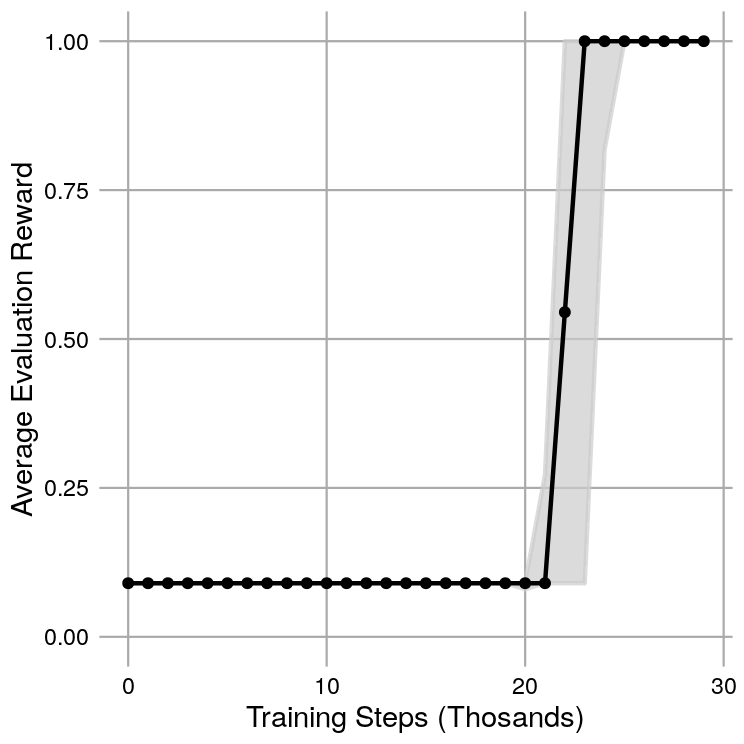
\includegraphics[scale=0.5]{DQNCorridor.png}
    }
    \subfloat[BNIG DQN]{
        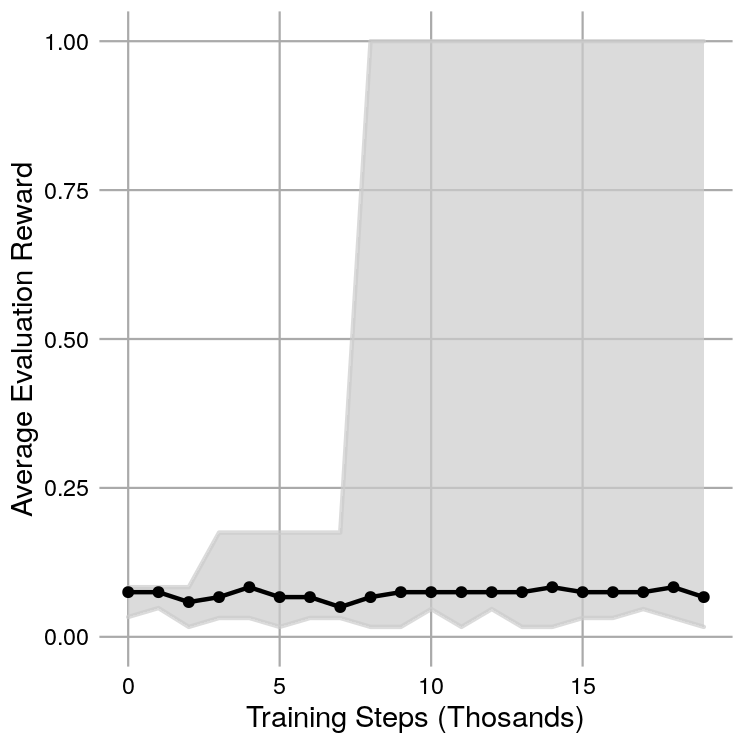
\includegraphics[scale=0.5]{BDQNCorridor.png}
    }
    \caption{\textbf{DQN and BNIG DQN Performance on Corridor}: Plots show the median performance over 10 different attempts. The shaded area covers 80\% of the total reward over all attempts.}
    \label{fig:nn_cartpole}
\end{figure}
\subsection{Cartpole}

The environment considered is a classic toy example called cartpole. The environment was first proposed in \cite{barto_sutton_1983} and is easily available through the Open AI gym environment \citep{brockman_2016}.
\todo figure to illustrate 
The task consists of balancing a pole on top of a cart. If the pole falls over 15 degrees from the upright position or if the cart goes too far (2.4 units from the center) to the left or right the game is terminated. The game is also terminated after 500 timesteps. Every timestep a reward of $+1$ is received. There are two actions, the cart can be pushed to the left or to the right at every timestep. There are 4 input variables that define the state: the pole angle from vertical, the position of the cart and the derivative of both variables. 

The environment implementation from OpenAI Gym was used \citep{OpenAI_gym}. Each method was run for 50,000 steps with 10 different seeds and every 1000 steps an evaluation phase is run over 1000 steps. The results are summarized in figure \ref{fig:nn_cartpole}.

\begin{figure}[H]
    \centering
    \subfloat[DQN]{
        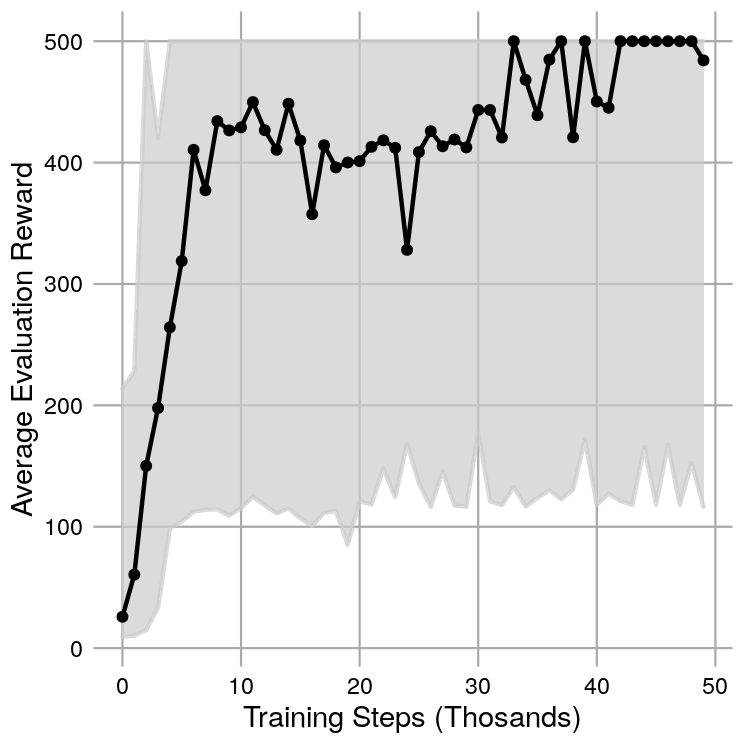
\includegraphics[scale=0.5]{DQNCartpole.png}
    }
    \subfloat[BNIG DQN]{
        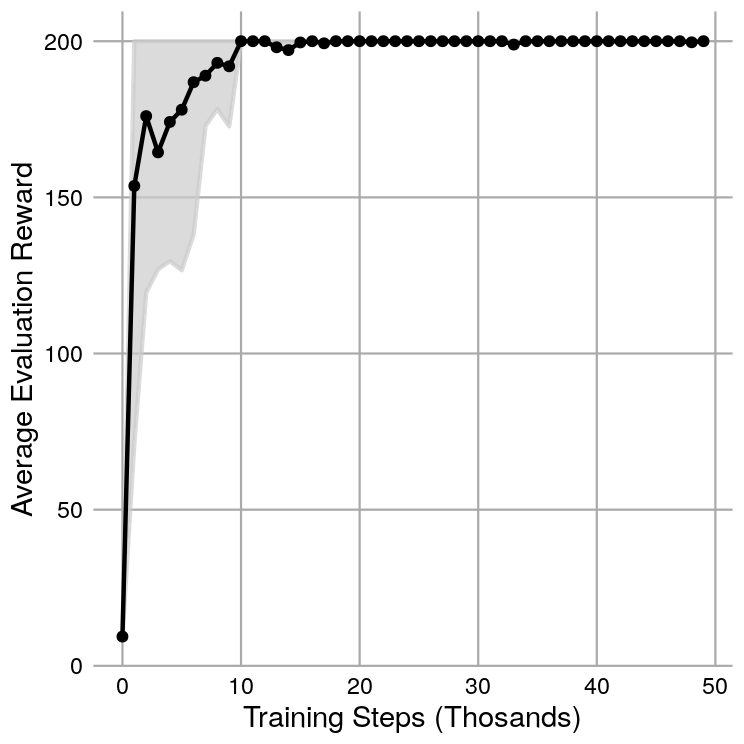
\includegraphics[scale=0.5]{BDQNCartpole.png}
    }
    \caption{\textbf{DQN and BNIG DQN Performance on Cartpole}: Plots show the median performance over 10 different attempts. The shaded area covers 80\% of the total reward over all attempts.}
    \label{fig:nn_cartpole}
\end{figure}

A policy that does not balance the pole lasts about 10 to 20 frames which is equivalent to a reward of 10 to 20. Figure \ref{fig:nn_cartpole} shows both methods are able to find successfull balancing policy. However, while the max performance of the DQN matches the BNIG DQN, the latter acheives much more stable results. Breaking down the results per seeds (figure \ref{fig:nn_per_cartpole}) one can see that the spread is caused by the instability of DQN after having found an optimal policy in some attempts and failing to find the optimal policy in others. The BNIG BDQN however always finds the optimal policy however can face some detoriation in performance towards the end of the experiment. 

\subsection{Acrobot}

Another common toy example is called acrobot. The experiment is first described in \cite{hauser_1990} and put into an RL context in \cite{sutton_1996}. The environment consists of a robot arm with two joints, one fixed to the origin and one with an actuator. The arm starts hanging downwards under the origin. The goal is to get the end of the robot arm over a line above the origin which terminates the episode. A reward of $-1$ is given each timestep. There are three actions, apply 1 torque left, 1 torque right or no operation. The state input is

$$
[\cos(\theta_1), \sin(\theta_1), \cos(\theta_2), \sin(\theta_2), \dot{\theta}_1, \dot{\theta}_2]
$$

where $\theta_1$ is the angle of the first joint and $\theta_2$ is the angle of the second joint relative to the first.

\todo figure to illustrate 

The environment implementation from OpenAI Gym was used \citep{OpenAI_gym}. Each method was run for 100,000 steps with 10 different seeds and every 2000 steps an evaluation phase is run over 2000 steps. 

\begin{figure}[H]
    \centering
    \subfloat[DQN]{
        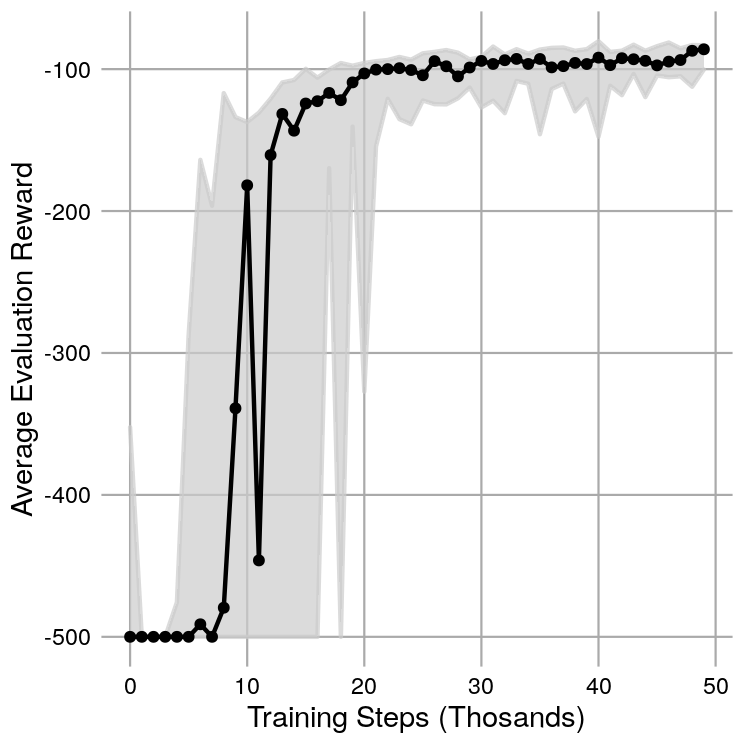
\includegraphics[scale=0.5]{DQNAcrobot.png}
    }
    \subfloat[BNIG DQN]{
        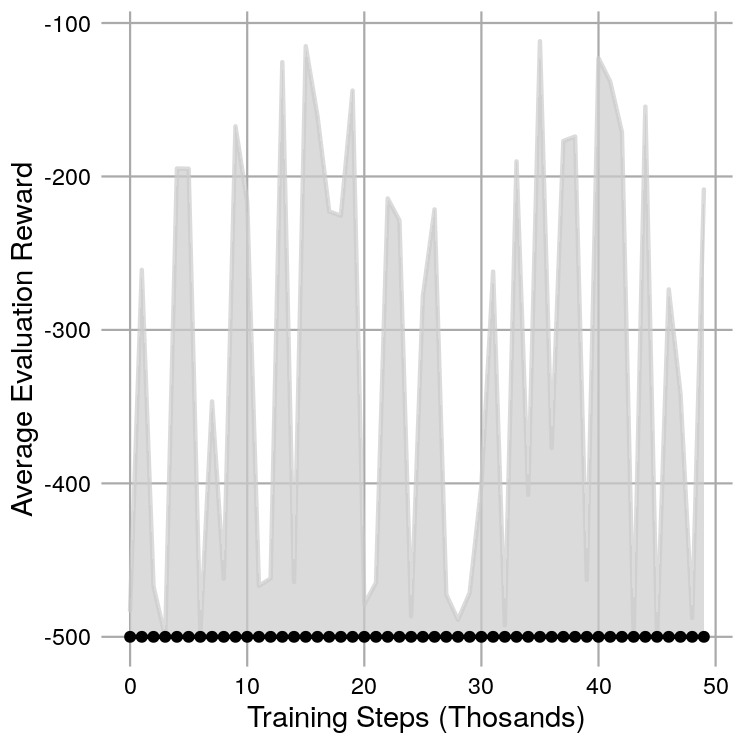
\includegraphics[scale=0.5]{BDQNAcrobot.png}
    }
    \caption{\textbf{DQN and BNIG DQN Performance on Acrobot}: Plots show the median performance over 10 different attempts. The shaded area covers 80\% of the total reward over all attempts.}
    \label{fig:nn_acrobot}
\end{figure}

A score above -500 indicates the agent was able to lift the robot arm over the required threshold. As seen in figure \ref{fig:nn_acrobot} both agents manage to do this. However, while the DQN model find a stable policy leading to an average reward of -100, the BDQN struggles to stay above -500. A deeper look into the per seed results (figure \ref{fig:nn_acrobot}) shows that the BDQN acheives an average reward of around -100 every seed. However, it is unable to keep this policy over more than two iterations before falling to a -500 reward again. There are many possible reasons. I can be caused by a too high learning rate, a miscalibrated exponential memory or a miscalibrated target update time period to a name a few.

\todo Try some hyperparameter tuning to get BNIG to work on acrobot. I have not been successfull with this yet. Maybe there is another reason this is failing? Note that this worked well when the bayesian regression was trained from scratch. UPDATE: Works with a higher alpha but this feels like just pushing the method towards a DQN. With a large alpha relative beta the noise term "disappears".

\subsection{Atari}

A standard benchmark in the deep RL field is a large set of atari 2600 games introduced in \cite{bellemare_13}. Papers presenting new methods in this field generally test on 40-50 of these games, such as in \cite{mnih_2015}, \cite{mnih_2016} and \cite{donoghue_2017}. However these algorithms are heavy to run, often taking close to a week on a GPU per game. Due to limited compute the BNIG DQN was tested once a subset of these games. The results were compared to 5 seeds of DQN runs that can be found in the Dopamine package. Both methods use all the same hyperparameters with the exception of the update horizon, which was set to 5 for the BNIG DQN. This is known to increase the performance of the DQN, so the results are not a completely fair comparison.

\subsubsection{Pong}

\begin{figure}[H]
    \centering
    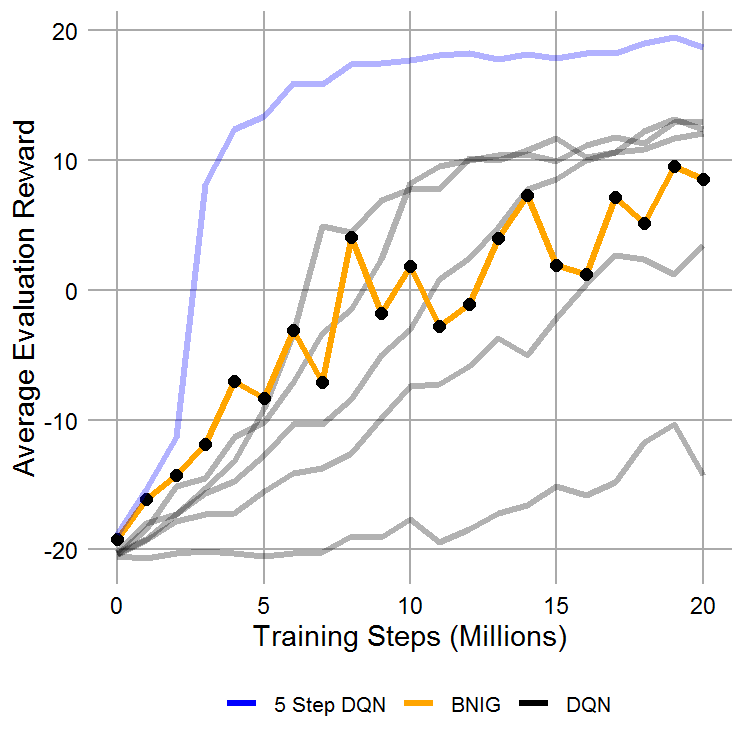
\includegraphics[scale=0.5]{BDQNPong.png}
    \caption{\textbf{BNIG DQN Performance on Pong}: Single seed BNIG DQN compared to 5 DQN seeds provided in the Dopamine package.}
    \label{fig:nn_pong}
\end{figure}

\todo Still running. Note I've used 50k steps for evaluation instead of 125K as in dopamine. So the results are a bit noisy due to this, but I don't think they are noisy enough to explain the observered behaviour.
\cleardoublepage